\chapter{Restauraci\'on de Imágenes}\label{chapter:ImIp} % II = Image Inpainting

\begin{definition}\label{def:inpainting}
	El problema de \II\footnote{T\'ermino en ingl\'es cuyo equivalente en el \'ambito del procesamiento de im\'agenes es \textit{restauraci\'on}.}, o en general el problema de \textit{inpainting} es el de recuperar una señal a partir de una versi\'on corrupta de la misma. Sea $\y$ un vector de dimensiones $m \times 1$ y $\z$ la versi\'on corrupta de $\y$ que le faltan algunos elementos, se tiene que:
	\begin{equation}
		z = My
		\label{eq:inpainting}
	\end{equation}
	donde $\mathbf{M}$ es una matriz diagonal de $m \times m$ con solo $0$'s y $1$'s la cual define las posiciones de los elementos faltantes. Se quiere encontrar el vector $\y$, cuando $\z$ y  $\mathbf{M}$ son conocidos. 
\end{definition}

Se ha de destacar que estamos en presencia de un problema mal planteado pues la $y$ buscada que satisface (\ref{eq:inpainting}) hay m\'as de una (en el caso del problema general sin restricciones, hay infinitas). Entre las dis\'imiles soluciones se busca la que bajo criterios subjetivos del ojo humano es la que mejor rellena las partes faltantes. La restauraci\'on en este trabajo se realiza sobre las im\'agenes digitales, en el siguiente ep\'igrafe se exponen sus principales características y como adaptarlas al problema anteriormente planteado. 

\section{Las im\'agenes digitales}\label{sec:digital_images}
Una imagen digital \cite{solomon2011fundamentals,enwiki:di,eswiki:id} es una representaci\'on bidimensional de una imagen, compuesta por elementos usualmente llamados \textit{p\'ixeles} que contienen informaci\'on finita en valores discretos que representan num\'ericamente la intensidad de alg\'un color o su escala de gris. Estos valores son la salida de una funci\'on en dos dimensiones cuyo dominio son coordenadas espaciales. La resolución de una imagen digital son aquellos intervalos de valores admisibles para cada coordenada espacial. En dependencia de si estos intervalos son fijos o din\'amicos la im\'agenes digitales se clasifican respectivamente en:
\begin{itemize}
	\item \textbf{Imagen matricial o mapa de bits} (conocido en ingl\'es como \textit{raster image} o \textit{bitmap}). Este tipo de imagen suele tener asociada una representaci\'on matricial, la cual es el resultado de tabular\footnote{Entiéndase por tabular una funci\'on $f$ al proceso de colocar en la posici\'on $i,\;j$ de la matriz el resultado de $f(i, j)$} la funci\'on que arroja el valor de los p\'ixeles. Comúnmente los píxeles contienen el valor de color o intensidad de la imagen que representa una muestra puntual de luz de una escena. La mayor\'ia de los formatos de archivos de im\'ages presentes en los diferentes dispositivos digitales hoy en d\'ia se usan para almacenar este tipo de im\'agenes \cite{eswiki:imp}.
	\item \textbf{Imagen o gr\'afico vectorial}. Basa su representaci\'on en el concepto geom\'etrico de vector y los elementos que contiene son tambi\'en otros conceptos geom\'etricos b\'asicos tales como los rectas, segmentos, pol\'igonos, circunferencias, arcos, elipses, \textit{etc}. Estos elementos traen consigo otros metadatos tales como el grosor de la linea y color del borde e interior. Este tipo de im\'agenes no se suele usar para capturar escenas reales, en cambio es m\'as \'util para representar logotipos, texto escrito, f\'ormulas y figuras matem\'aticas. Una de sus principales ventajas es su escalabilidad a cualquier tamaño de marco donde se muestre, pues su cencepci\'on geom\'etrica permite \textit{dibujarla} sin perder ning\'un nivel de detalle \cite{eswiki:igv}.
\end{itemize}

Las imágenes digitales se pueden obtener de varias formas. Por medio de dispositivos de entrada conversión analógica-digital como los escáneres y las cámaras digitales. Directamente mediante programas informáticos editores de mapas de bits y dibujo vectorial, como por ejemplo realizando dibujos con el ratón o tableta digitalizadora gráfica incluyendo el lápiz óptico, por otro lado mediante un programa de renderización 3D a mapa de bits. Luego de que se obtienen su informaci\'on pasa usualmente por un proceso de serializaci\'on y luego compresi\'on que se almacena en determinado formato digital. La mayoría de formatos de imágenes digitales están compuestos por una cabecera que contiene atributos (dimensiones de la imagen, tipo de codificación, \textit{etc}.), seguida de los datos de la imagen en sí misma. La estructura de los atributos y de los datos de la imagen es distinto en cada formato. Además, los formatos actuales añaden a menudo una zona de metadatos (escala de sensibilidad, flash, \textit{etc}.) Estos metadatos se utilizan muy a menudo en el formato extensión para cámaras digitales y videocámaras.

\subsection{Las im\'agenes matriciales}

Tal y como se expresa en la definici\'on del problema de restauraci\'on de im\'agenes (definici\'on \ref{def:inpainting}), se trata de im\'agenes representables como una señal o vector. El caso m\'as conveniente son las im\'agenes matriciales pues se pueden vectorizar de manera trivial. En este trabajo no se tratar\'a el caso de las im\'agenes vectoriales debido a que no est\'a claro su adaptaci\'on para el problema de la restauraci\'on. El análisis ir\'a enfocado en aquellas im\'agenes digitales con alg\'un tipo de representaci\'on matricial.

La imagen matricial o mapa de bits est\'a compuesta por una matriz $\I_{a \times b}$ con $a$ filas y $b$ columnas. Cada elemento o p\'ixel de dicha matriz suele ser un valor escalar o una tupla de escalares, que como se ha mencionado anteriormente representan la intensidad de un color o de la luz en sus coordenadas. En el caso más simple, cada píxel contiene un único valor numérico que representa el nivel de intensidad de la señal en ese punto de la imagen. Para convertir estos escalares a un elemento visual se usa un mapa de colores, el cual asigna un tono de color especifico a cada uno de los valores en un intervalo discreto y finito. Dicho intervalo contiene todos los valores v\'alidos que pueden tomar los p\'ixeles de la imagen.

El mapa de colores más comúnmente usado es la escala de grises, que asigna todos los matices de gris desde el negro (valor $0$) hasta el blanco (máximo valor del intervalo) según el nivel de la señal. El intervalo de valores estándar es $[0,\; 255]$, considerando solo los n\'umeros enteros. Son un total de $256$ n\'umeros en ese intervalo, que es justamente la m\'axima cantidad de enteros que se puede almacenar en 8 bits. La escala de grises se adapta especialmente bien a las imágenes que expresan sólo la intensidad de la señal como un valor único en cada punto de la región.
\begin{figure}[h]
	\centering
	\begin{tikzpicture}
		\node (image) at (0,0) {
\includegraphics[width=0.75\textwidth,height=1cm]{Graphics/colormap_gray.png}};
		\coordinate (a) at ($(image.south west)+(0.15, 0)$);
		\coordinate (b) at ($(image.south east)+(-0.15, 0)$);
		\draw[-] (a) -- (b);
		\draw[-] (a) -- ++(0, -.25) node[below]{0};
		\draw[-] ($(a)!0.25!(b)$) -- ++(0, -.25) node[below]{63};
		\draw[-] ($(a)!0.50!(b)$) -- ++(0, -.25) node[below]{127};
		\draw[-] ($(a)!0.75!(b)$) -- ++(0, -.25) node[below]{191};
		\draw[-] (b) -- ++(0, -.25) node[below]{255};
	\end{tikzpicture}
	\caption{Mapa de color de la escala de grises}
\end{figure}

\subsection{Mapa de color RGB}

Además de las imágenes en escala de grises, existen imágenes en color en las que el espectro completo de colores puede representarse como una terna de escalares. La forma est\'andar es mediante los componentes \RGB\footnote{Por sus siglas en ingl\'es \textit{red, green and blue}: rojo, verde y azul} en cada píxel. El color se representa como una combinación lineal de los colores primarios de la luz, cada elemento de la terna indica la intensidad de rojo, verde o azul necesarios para formar el color en cuesti\'on. Las im\'agenes \RGB pueden ser vistas de tres formas distintas:
\begin{itemize}
	\item Como un arreglo tridimensional.
	\item Como una matriz cuyos elementos son ternas.
	\item Como una terna de matrices de igual dimensi\'on.
\end{itemize}
En el \'ultimo caso a cada matriz se le llama \textit{canal}, por ejemplo el \textit{canal rojo} es la matriz que contiene los valores de las intensidades de rojo.

El espacio de color \RGB se basa en la porción del espectro electromagnético perceptible por los humanos para cada una de las longitudes de onda de los colores rojo, verde y azul. An\'alogo a la escala de grises las intensidades en cada canal toman valores enteros en el intervalo $[0,\; 255]$ y a mayor es el valor mayor es la intensidad en el color resultante. De modo que el rojo se obtiene con $(255,0,0)$, el verde con $(0,255,0)$ y el azul con $(0,0,255)$

Para este trabajo se tomar\'a como convenio que cuando se trata de la imagen como matriz se refiere en el caso de la escala de grises a su matriz de intensidades. En el caso de im\'agenes como las \RGB se refiere a alguno de sus canales. Si se quiere realizar la restauraci\'on a una imagen representada en varios canales de color, se aplica la restauraci\'on a cada uno de estos de forma independiente, luego la imagen final restaurada tendr\'a como canales esos que se restauraron.


\section{Los parches de una imagen}\label{sec:patches}

\begin{definition}
	Un parche  de una imagen (matriz) dada no es m\'as que una subimagen (submatriz) cuadrada de dimensiones $\sqrt{n} \times \sqrt{n}$. El tamaño del parche es $n$ y usualmente es muy peque\~no comparado con las dimensiones de la imagen.
\end{definition}

\begin{figure}[h]
	\centering
	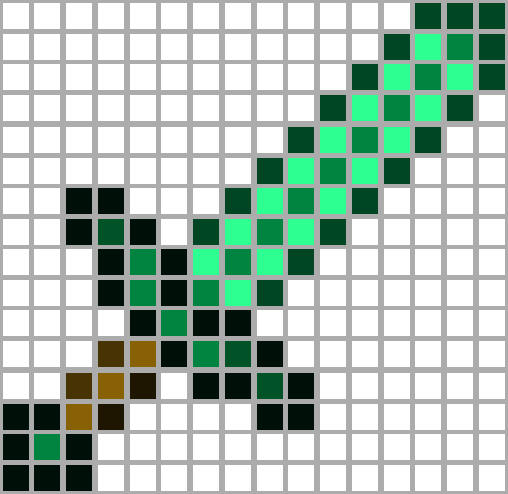
\includegraphics[width=4cm, height=4cm]{Graphics/diamon_sword.png}
	\hspace{1cm}
	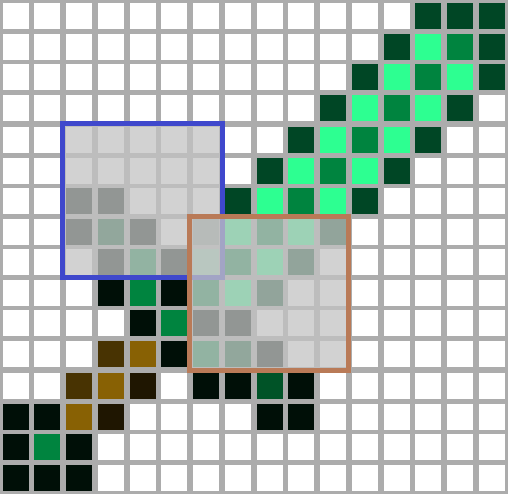
\includegraphics[width=4cm, height=4cm]{Graphics/diamon_sword_with_patches.png}
	\caption{Una imagen de $16 \times 16$ y dos parches de esta tomando $n = 25$.}
	\label{ex:patches}
\end{figure}

En la figura \ref{ex:patches} se ejemplifica visualmente el concepto de parches. Como vemos estos pueden solaparse sin ning\'un problema. Es de inter\'es en el siguiente cap\'itulo el conjunto de todos los parches, incluyendo con solapamientos.

\begin{lemma}\label{le:count_patches}
	La cantidad de parches de una matriz (imagen) incluyendo los solapamientos, para una matriz $A$ de dimensiones $a \times b$, y tomando los parches de $\sqrt{n} \times \sqrt{n}$, es igual a:
	
	\begin{equation}
		(a - \sqrt{n} + 1)(b - \sqrt{n} + 1)
		\label{eq:count_patches}
	\end{equation}
\end{lemma}


\textbf{Demostraci\'on:} tomando como referencia la esquina superior izquierda de un parche, esta solo puede ser ubicada verticalmente en el intervalo de posiciones \\$[1,\; a - \sqrt{n} + 1]$, de lo contrario el parche sobresaldr\'ia de la imagen. An\'alogamente solo puede ser colocado horizontalmente en el intervalo de posiciones $[1,\; b - \sqrt{n} + 1]$. Aplicando el principio combinatorio de la multiplicaci\'on, un parche puede ser ubicado de $(a - \sqrt{n} + 1)(b - \sqrt{n} + 1)$ formas distintas $\blacksquare$.

\begin{lemma}\label{le:count_patches_ieq}
	La cantidad de parches con solapamiento de una matriz A, con $n > 1$, es menor que la cantidad de elementos de la misma.
\end{lemma}

\textbf{Demostraci\'on:} Sea $A$ de $a \times b$; dado que $n > 1$ se cumple la siguiente desigualdad:

\begin{equation}
	\begin{array}{lrcl}
		                &               1 &<& n        \\ 
		\Longrightarrow &               1 &<& \sqrt{n} \\
		\Longrightarrow &   -\sqrt{n} + 1 &<& 0        \\
		\Longrightarrow & a -\sqrt{n} + 1 &<& a        \\
	\end{array}
\end{equation}

An\'alogamente $b -\sqrt{n} + 1 < b$, multiplicando las dos desigualdades obtenemos:

\begin{equation}
	(a - \sqrt{n} + 1)(b - \sqrt{n} + 1) < ab
	\label{eq:count_patches_ieq}
\end{equation}

Por el lema \ref{le:count_patches} la cantidad de parches de A es $(a - \sqrt{n} + 1)(b - \sqrt{n} + 1)$ lo que es menor que $ab$ $\blacksquare$.

\begin{definition}
	El p\'ixel o elemento central de un parche es aquel que se encuentra en una posici\'on prefijada, dicha posici\'on debe ser la misma para todos los parches de una misma imagen.
\end{definition}

\begin{figure}[h]
	\centering
	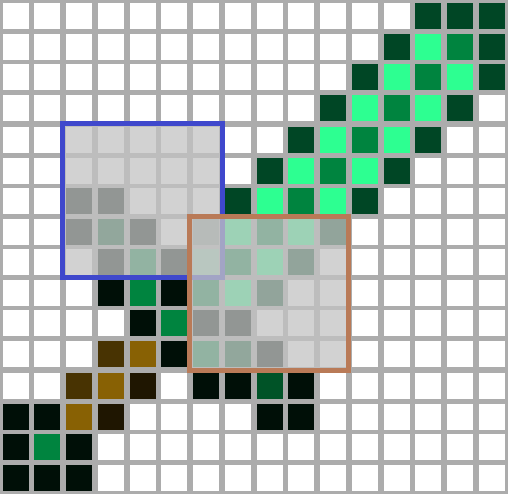
\includegraphics[width=4cm, height=4cm]{Graphics/diamon_sword_with_patches.png}
	\hspace{1cm}
	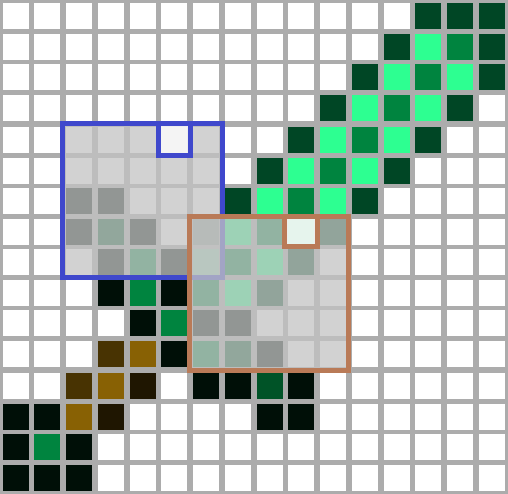
\includegraphics[width=4cm, height=4cm]{Graphics/diamon_sword_with_patches_and_centers.png}
	\caption{Parches con p\'ixel central (marcado en rojo) situado en la posici\'on $(1,\;4)$.}
	\label{ex:patch_center}
\end{figure}

En la figura \ref{ex:patch_center} se muestran los centros de los parches del ejemplo anterior. No debemos confundir el p\'ixel central con aquel que se encuentra en su centro geom\'etrico. La idea de este elemento es para tomarlo como punto de referencia o representativo. Un ejemplo se ve en el cap\'itulo \ref{chapter:SCHEME}, como para aquellos p\'ixles que no se conoce su valor, se usa en cambio el parche del cual ellos son su centro.

\section{Señales y vectorizaci\'on de matrices}\label{sec:signals}

Para adaptar las im\'agenes con representaci\'on matricial al problema de la restauraci\'on (definición \ref{def:inpainting}) es necesario transformar su respectiva matriz a un vector o señal. En el entorno matem\'atico, específicamente en \'algebra linear \cite{enwiki:la} la vectorizaci\'on de una matriz es una transformaci\'on linear la cual convierte una matriz a un vector columna.
\begin{definition}
	Sea la matriz $A_{m \times n} = \{a_{i,j}\}$, se define como su vectorizaci\'on al vector denotado por $vec(A)$, de dimensi\'on $mn \times 1$ que resulta de apilar las columnas de $A$ de la siguiente forma:
	\begin{equation*}
		vec(A) = \left(
		\begin{array}{ccccccc}
		a_{1,1}&a_{2,1}\;\cdots\;a_{m,1}&a_{1,2}&a_{2,2}\;\cdots\;a_{m,2}&\cdots&a_{1,n}&a_{2,n}\;\cdots\;a_{m,n}\\
		\end{array} \right)^\intercal
	\end{equation*}
\end{definition}
Para obtener la vectorizaci\'on de las filas de $A$, se debe simplemente vectorizar su transpuesta: $vec(A^\intercal)$. El siguiente ejemplo muestra tanto vectorizaci\'on por columnas, como por filas.
\begin{figure}[h]
	\[
		A = \left(
		\begin{matrix}
			23 & 14 & 9\\
			90 & -54 & -2\\
		\end{matrix}\right)
		\qquad
		vec(A) = \left(
		\begin{matrix}
			23\\
			90\\
			14\\
			-54\\
			9\\
			-2\\
		\end{matrix}\right)
		\qquad
		vec(A^\intercal) = \left(
		\begin{matrix}
			23\\
			14\\
			9\\
			90\\
			-54\\
			-2\\
		\end{matrix}\right)
	\]
	\label{ex:vectorization}
	\caption{Vectorizaci\'on para una matriz de $2 \times 3$}
\end{figure}

Los conceptos de vector y señal son muy similares, y en este trabajo se usan ambos t\'erminos indistintamente para referirse a lo mismo. A continuaci\'on se expone su equivalencia.
\begin{definition}
	Una señal se define como una secuencia de n\'umeros reales ordenados en el tiempo de forma discreta. En otras palabras una señal es una función $s$:
	\begin{equation}
		s : \mathbb{N}^\ast \rightarrow \mathbb{R}
	\end{equation}
	donde $s(t)$ es el $t$-\'esimo elemento de la señal y $t$ su tiempo representado como un entero. 
\end{definition}
\begin{definition}
	Una señal finita $s$ de tamaño $m$ es aquella cuyo dominio se restringe al intervalo de los primeros $m$ enteros positivos:
	\begin{equation}
		s : [1,\;m] \rightarrow \mathbb{R}
	\end{equation}
\end{definition}
La equivalencia entre vectores y señales es trivial. Sea $V = \{v_i\}$ un vector, su señal equivalente $S_V$ es aquella tal que $S_V(i) = v_i$ para todo $i$. Por lo tanto el conjunto de las señales finitas de tamaño $m$ coincide con el espacio vectorial de dimensi\'on $m$, y el conjunto de las señales infinitas coincide con el espacio vectorial de dimensi\'on infinita. Luego para los prop\'sitos de este trabajo tanto \textit{vector} como \textit{señal} significan lo mismo.

Finalmente se hace necesario tratar el tema de la suavidad de una señal, pues se usar\'a m\'as adelante en el cap\'itulo \ref{chapter:SCHEME}. Este concepto no es m\'as que la percepci\'on visual de que tan suave es la gr\'afica de la señal en el plano cartesiano. Como se trata de algo subjetivo se usa en su lugar medidas aceptadas en la literatura, para este trabajo se usa la medida de varianza total: \textbf{TV}\footnote{Por sus siglas en ingl\'es: \textit{total variance}}.
\begin{definition}\label{def:tv}
	La varianza total de una señal $s$ se define como:
	\begin{equation}
		\|s\|_{TV} = \sum_{i}|s(i) - s(i - 1)|
	\end{equation}
\end{definition}

\section{Matrices de permutaci\'on}\label{sec:permutation_matrices}

La permutación de filas y/o columnas de una matriz es una operación muy frecuente en la implementación de técnicas directas o iterativas sobre estas. En este trabajo se hace uso de las matrices de permutaci\'on, de ah\'i la relevancia de las siguientes definiciones:

\begin{definition}\label{def:permutation}
	Sea $A_{m \times m} = \{a_{i,j}\}$ una matriz y $\pi = \{i_1,\; i_2,\; \dots,\; i_m\}$ una permutaci\'on del conjunto $\{1,\; 2,\; \dots,\; m\}$. Entonces las matrices:
	\begin{equation}
		\begin{array}{c}
			A_{\pi,\ast} = \{a_{\pi(i),j}\}\quad i=\overline{1,n}; \quad j=\overline{1,n}\\
			\\
			A_{\ast,\pi} = \{a_{i,\pi(j)}\}\quad i=\overline{1,n}; \quad j=\overline{1,n}\\
		\end{array}
	\end{equation}
	se llaman $\pi$-permutaci\'on de filas y $\pi$-permutaci\'on de columnas respectivamente.
\end{definition}

Es bien conocido que cualquier permutación $\pi$ resulta de una sucesi\'on de intercambios. Por ejemplo, permutaciones elementales en las cuales solo dos elementos se intercambian. Una matriz de intercambio es una matriz identidad con dos de sus filas intercambiadas. Denotemos por $C_{i,j}$ tales matrices con $i$ y $j$ los números de las filas intercambiadas. Note que para intercambiar las filas $i$ y $j$ de $A$ solo necesitamos premultiplicarla por la matriz $C_{i,j}$.

Sea $\pi$ una permutación arbitraria. Esta permutación es el resultado de la secuencia de $\sigma(i_k, j_k),\; k=\overline{1,m}$ intercambios consecutivos. Entonces las filas de una matriz pueden ser permutadas intercambiando las filas $(i_1, j_1)$, después las $(i_2, j_2)$ de la matriz resultante, as\'i sucesivamente y finalmente intercambiando $(i_m, j_m)$ de la \'ultima matriz. Cada una de estas operaciones puede ser realizada premultiplicando $A$ por $C_{i_k, j_k}$. La misma operación puede realizarse teniendo en cuenta las columnas de una matriz: para intercambiar las columnas $i$ y $j$ de una matriz la postmultiplicamos por $C_{i,j}$.
\begin{lemma}\label{lm:dual_permutation}
	Sea $A_{m \times m} = \{a_{i,j}\}$ una matriz y $\pi$ la permutación resultante del producto de los intercambios $\sigma(i_k, j_k),\; k=\overline{1,m}$, entonces:
	\begin{equation}
		\begin{array}{rcl}
			A_{\pi,\ast} = P_\pi A &\mbox{donde}& P_\pi = C_{i_m, j_m}C_{i_{m-1}, j_{m-1}}\;\cdots\;C_{i_1, j_1}\\
			\\
			A_{\ast,\pi} = A Q_\pi &\mbox{donde}& Q_\pi = C_{i_1, j_1}C_{i_2, j_2}\;\cdots\;C_{i_m, j_m}\\
		\end{array}
	\end{equation}
	Los productos de matrices de intercambio $P_\pi$ y $Q_\pi$ se llaman matrices de permutación.
\end{lemma}

\begin{definition}
	Una matriz de permutación no es otra cosa que una matriz identidad con sus filas y columnas permutadas.
\end{definition}

N\'otese que $C_{i, j}^2 = \I$ es decir, el cuadrado de una matriz de intercambio es igual a la identidad. Por lo que la inversa de una matriz de intercambio es igual a sí misma $C_{i, j} = C_{i, j}^{-1}$. Usando estos resultados es fácil ver que las matrices $P_\pi$ y $Q_\pi$ satisfacen que:
\begin{equation}
	P_\pi Q_\pi = C_{i_m, j_m}C_{i_{m-1}, j_{m-1}}\;\cdots\;C_{i_1, j_1} C_{i_1, j_1}C_{i_2, j_2}\;\cdots\;C_{i_m, j_m} = \I
	\label{eq:dual_permutation}
\end{equation}
lo cual muestra que las dos matrices $P_\pi$ y $Q_\pi$ son no singulares y una es la inversa de la otra. En otras palabras permutar las filas y las columnas de una matriz usando la misma permutación es una transformación de semejanza.

\begin{lemma}\label{lm:inverse_permutation}
	La matriz inversa de una matriz de permutaci\'on $P_\pi$ es su transpuesta y por tanto es ortogonal:
	\begin{equation}
		P_\pi^{-1} = P_\pi^\intercal
	\end{equation}
\end{lemma}
\textbf{Demostraci\'on}: usando el lema \ref{lm:dual_permutation} con $A = \I_{m \times m}$ se obtiene que $\I_{\pi,\ast} = P_\pi$ y $\I_{\ast,\pi} = Q_\pi$. Ahora bien $\I_{\pi,\ast}$ es la $\pi$-permutaci\'on por filas de la matriz identidad, por tanto su transpuesta $\I_{\pi,\ast}^\intercal$ es la $\pi$-permutaci\'on por columnas. Luego:
\begin{equation*}
	\def\arraystretch{1.5}
	\begin{array}{rrcl}
		&\I_{\pi,\ast}^\intercal &=& \I_{\ast,\pi}\\
		\Longrightarrow&P_\pi^\intercal &=& Q_\pi\\
		\overset{(\ref{eq:dual_permutation})}{\Longrightarrow}&P_\pi^\intercal &=& P_\pi^{-1} \quad\blacksquare\\
	\end{array}
\end{equation*}
